
\section{Charm and kaon physics}

\label{sec:CharmAndKaon}
In the LHC collisions, a large part of the proton-proton cross section goes into charm and strange quarks production.  
The $c \bar{c}$ cross-section is roughly 10\% of the total inelastic cross-section, so that charm hadrons are produced extremely copiously. Their short but measurable decay times make them relatively simple to reconstruct and separate from background. The LHCb detector has developed dedicated triggers registering  large samples of charm hadron decays and is currently exploring the best strategy to collect a large quantity of kaon decays. In fact, charm and kaon physics provides complementary insights into flavour  physics to the ones obtained from the $b$ sector.  In the context of the GDR, we will profit of the previous experimental experience of the French community in these domains to try to extract the most of the physic potential for charm and kaon physics within LHCb, but we will of course follow the results of the currently ongoing dedicated experiments like NA62. Their is a clear interplay with the studies concerning $CP$ violation and rare decays in the charm and kaon sectors with those in the $b$ sector. Thanks to the GDR, the  community will  have the possibility to come together and analyze all the results of flavour  in a general framework. 

\subsection*{Charm physics}
 Theoretically, $CP$ violation in charm mesons is expected to be very small
because the GIM mechanism is much more powerful for $c\rightarrow u$
transitions than for $s\rightarrow d$ or $b\rightarrow s,d$ transitions. The $CP$ violation in decay is therefore expected to occur at below the per mil level in the SM.  
At the same time, NP need not to respect this peculiar feature, so these
observables provide almost-null tests of the SM.  
Additionally, compared to beauty or strange hadrons, the mixing of neutral charm hadrons is slow, with both the $x = \Delta m/\Gamma$ and $y = \Delta \Gamma/ (2\Gamma)$ parameters at around the percent level.

 The $CP$ violation in charm decays has not been observed so far, and the existing experimental limits are at the few per mil level. The theoretical predictions of charm $CP$ violation are difficult as long distance contributions dominate; $CP$ violation in decay close to the present experimental limits could be accommodated within the SM or could be signs of NP, and a progress on the theory side is required to disentangle the two. Similarly, in the case of mixing, or $CP$ violation in the interference of decay and mixing, more precise experimental results are needed to stimulate progress on the theoretical predictions. The current bounds are shown in figure~\ref{fig charm} on the left.

In addition, charmed hadrons are also an interesting place to study rare and forbidden transitions, for example flavour  changing neutral currents (FCNC) or lepton number violating decays. The most recent studies of charmed hadron decays within the French community were performed on the rare decays $D_{(s)}^+ \to \pi \mu\mu$~\cite{Aaij:2013sua} with same sign muons and $D^0 \to K \pi\mu\mu$~\cite{Aaij:2015hva}. The former is of interest because the copious production rate of charmed hadrons allows effective limits to be placed on Majorana neutrinos. The latter is the charmed counterpart of $B\to K^*\mu\mu$ and has now been observed for the first time by LHCb, albeit within a dimuon $q^2$ region dominated by the $\omega$ and $\rho$ resonances. It should in principle share much of the same phenomenology of $B\to K^*\mu\mu$,  with the complication of much higher backgrounds from decays to hadronic resonances (such as $\rho$) which subsequently decay to dimuon pairs. Once that a large signal yield becomes available, an angular analysis will be of prior interest. 

\subsubsection*{Plans for the GDR}
In the upcoming period, the most critical work  in the charm field will be the following.
\begin{itemize}
\item Improve the limits on $CP$ violation in charm, both in decay and the interference of mixing and decay, as well as  make ever more precise measurements of charm mixing parameters using both the $D\to hh$ and $D\to K_s hh$ decay modes with the full Run2  LHCb dataset. \item LHCb should obtain large samples of FCNC decays such as $D^0\to K \pi\mu\mu$.  Potentially this will allow for an observation of the non-resonant (in the dimuon spectrum) decay and a measurement of angular observables similar to the ones which characterise $B\to K^*\mu\mu$. 
\item Make more precise measurements of charm hadron lifetimes, in particular in the less well understood baryon sector. This could aid the development of heavy quark effective theory (HQE) tools and techniques required to eventually obtain precise SM predictions for mixing and $CP$ violation in the charm sector.
\end{itemize}



\subsection*{Kaon physics}

  Kaon physics is the birthplace of $CP$ violation, and has played a central
role in establishing the CKM picture in the past five decades. Kaon mixing and decays belong traditionally to the most constraining processes for physics beyond the SM. Currently, two main aspects are relevant for our proposed plans. First, advances in lattice QCD may well help to finally shed new light on the precisely measured direct $CP$ violation parameter $\epsilon^{\prime}_K$. Over the last years, lattice-QCD progress in the evaluation of $K \to \pi \pi$ matrix elements has been no less than astonishing. As a result, a mature, first-principle SM calculation of $\epsilon^\prime_K/\epsilon_K$ is no more just a dream. We should emphasize that this quantity, along with $\epsilon_K$ itself, is among the most formidable probes of physics beyond the SM, as it is able to probe NP scales as large as $10^{4}$ TeV. Second, theorists will be following closely the NA62 experiment, which aims at observing the ultra-rare and ultra-clean $K^{+}\rightarrow\pi ^{+}\nu\nu$ decay. The potential of this experiment, as well as of KOTO for the corresponding channel with a neutral pion, is shown in figure~\ref{fig charm} on the right.  Any hint of discrepancy with the SM in either of the $K$-physics quantities mentioned above would have implications for the other meson sectors.

In addition, the discrepancies found in recent LHCb and $B$-factory data, in particular in the quantity known as $R_K$ \cite{Aaij:2014ora}, provide motivations for searches of certain $K$ decays, in particular lepton-flavour violating  ones of the kind $K \to (\pi) e \mu$. In fact, $R_K$ may be naturally explained by a Fermi-like, TeV-scale new interaction involving third-generation quarks and leptons only \cite{Glashow:2014iga}. At the  energy scales of the decaying mesons, this interaction will produce, along with LFUV effects such as $R_K$, also LFV $B$ decays, whose natural magnitude can be estimated to be in the ballpark of $10^{-8}$ by just using the departure of $R_K$ from unity \cite{Glashow:2014iga}. That argument can be extended to $K$ decays as well, in particular those of the kind $K \to (\pi) \ell \ell'$ such as $K_L \to e^\pm \mu^\mp$ and $K^+ \to \pi^+ e^\pm \mu^\mp$. Limits on these modes are more than ten years old: $\mc B(K_L \to e^\pm \mu^\mp) < 4.7 \times 10^{-12}$ \cite{Ambrose:1998us}, $\mc B(K^+ \to \pi^+ e^- \mu^+) < 1.3 \times 10^{-11}$ \cite{Sher:2005sp}, $\mc B(K^+ \to \pi^+ e^+ \mu^-) < 5.2 \times 10^{-10}$ \cite{Appel:2000tc}. Theoretically, their expected magnitudes can be estimated after suitably normalizing them to cancel phase-space factors \cite{Cahn:1980kv}. The NP flavor structure can further be specified by using, for definiteness, flavor models proposed in connection with the $R_K$ result, e.g. \cite{Guadagnoli:2015nra,Boucenna:2015raa},   obtaining:
\be
\label{eq:KLemu}
\mc B(K_L \to e^\pm \mu^\mp) \approx 6 \times 10^{-14}~, \\
\mc B(K^+ \to \pi^+ e^\pm \mu^\mp) \approx 3 \times 10^{-15}~.
\ee
While the $K^+$ LFV mode is clearly too suppressed, the $K_L$ one has a branching ratio close to $10^{-13}$. Such a rate may actually well be reachable at the NA62 experiment. Concerning LHCb, it should be noted that, although $K$ mesons are produced copiously, their lifetimes are typically too long for the detector size, with the exception of the $K_S$. A dedicated study is thus necessary to understand the actual LHCb capabilities for the above decays.

\subsubsection*{Plans for the GDR}

The above considerations can be translated in a number of interesting directions to be pursued in the framework of the GDR.

\begin{itemize}

\item Closely follow the impressive progress in the lattice-QCD evaluation of direct and indirect CP violation in the kaon sector. The French community has a tradition in lattice QCD and in kaon physics, and can play a leading role in establishing possible discrepancies in the mentioned quantities, and in their interpretation.

\item The meetings organized in the context of the present GDR will allow to invite  members of the NA62 collaboration, giving the opportunity to have regular exchanges with them. In this way our network will  follow closely the progress in the search of the $K^+ \to \pi^+ \nu \bar \nu$ decay and of the LFV decays of $K$ mesons.

\item An open question is, as mentioned, the possible reach of LFV $K$ decays by LHCb itself. Optimistic remarks on this possibility actually emerged in informal discussions  preceding the writing of the present document. This possibility deserves a dedicated study, and the GDR will be instrumental to frame progress in this direction.

\end{itemize}



\begin{figure}[!htb]
\begin{center}
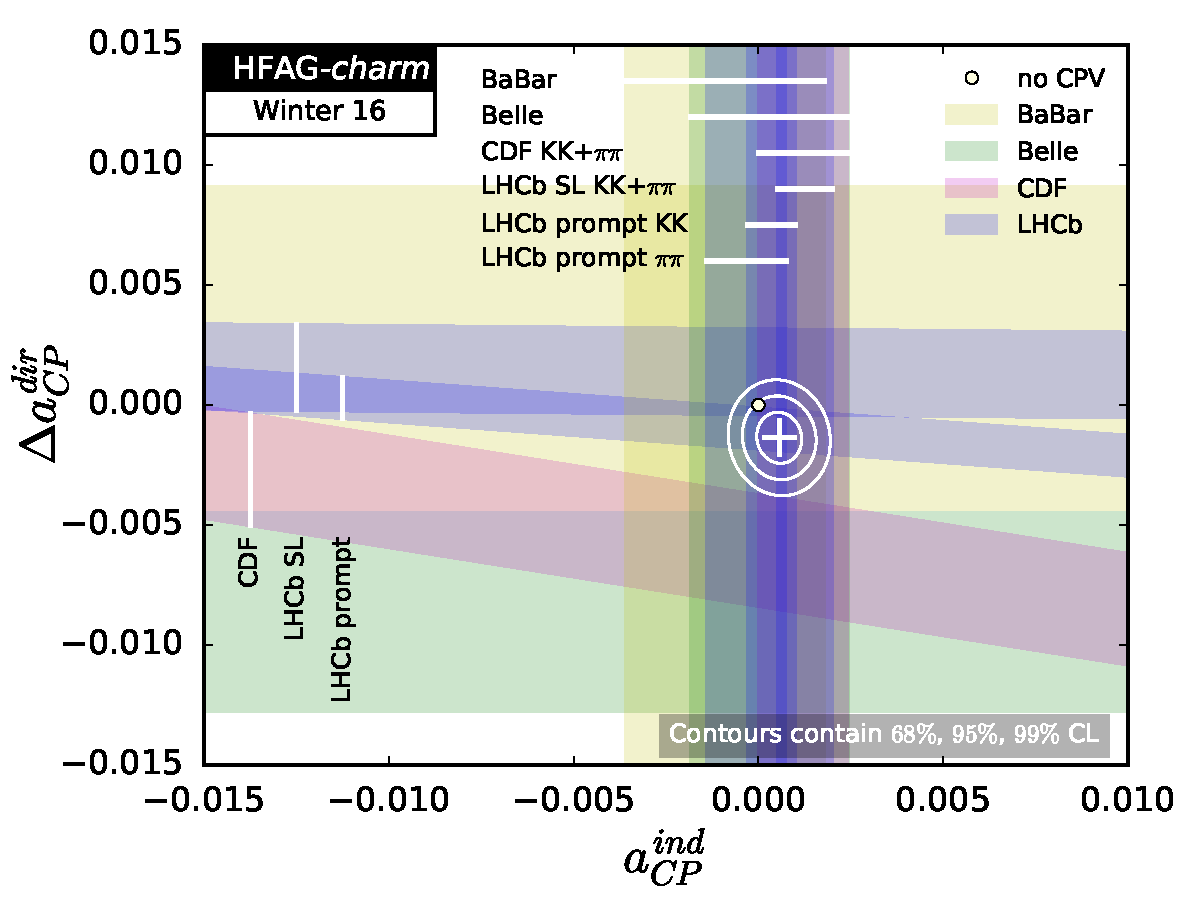
\includegraphics[width=7.5cm]{./deltaACP_AGamma_fit_Winter16.pdf}
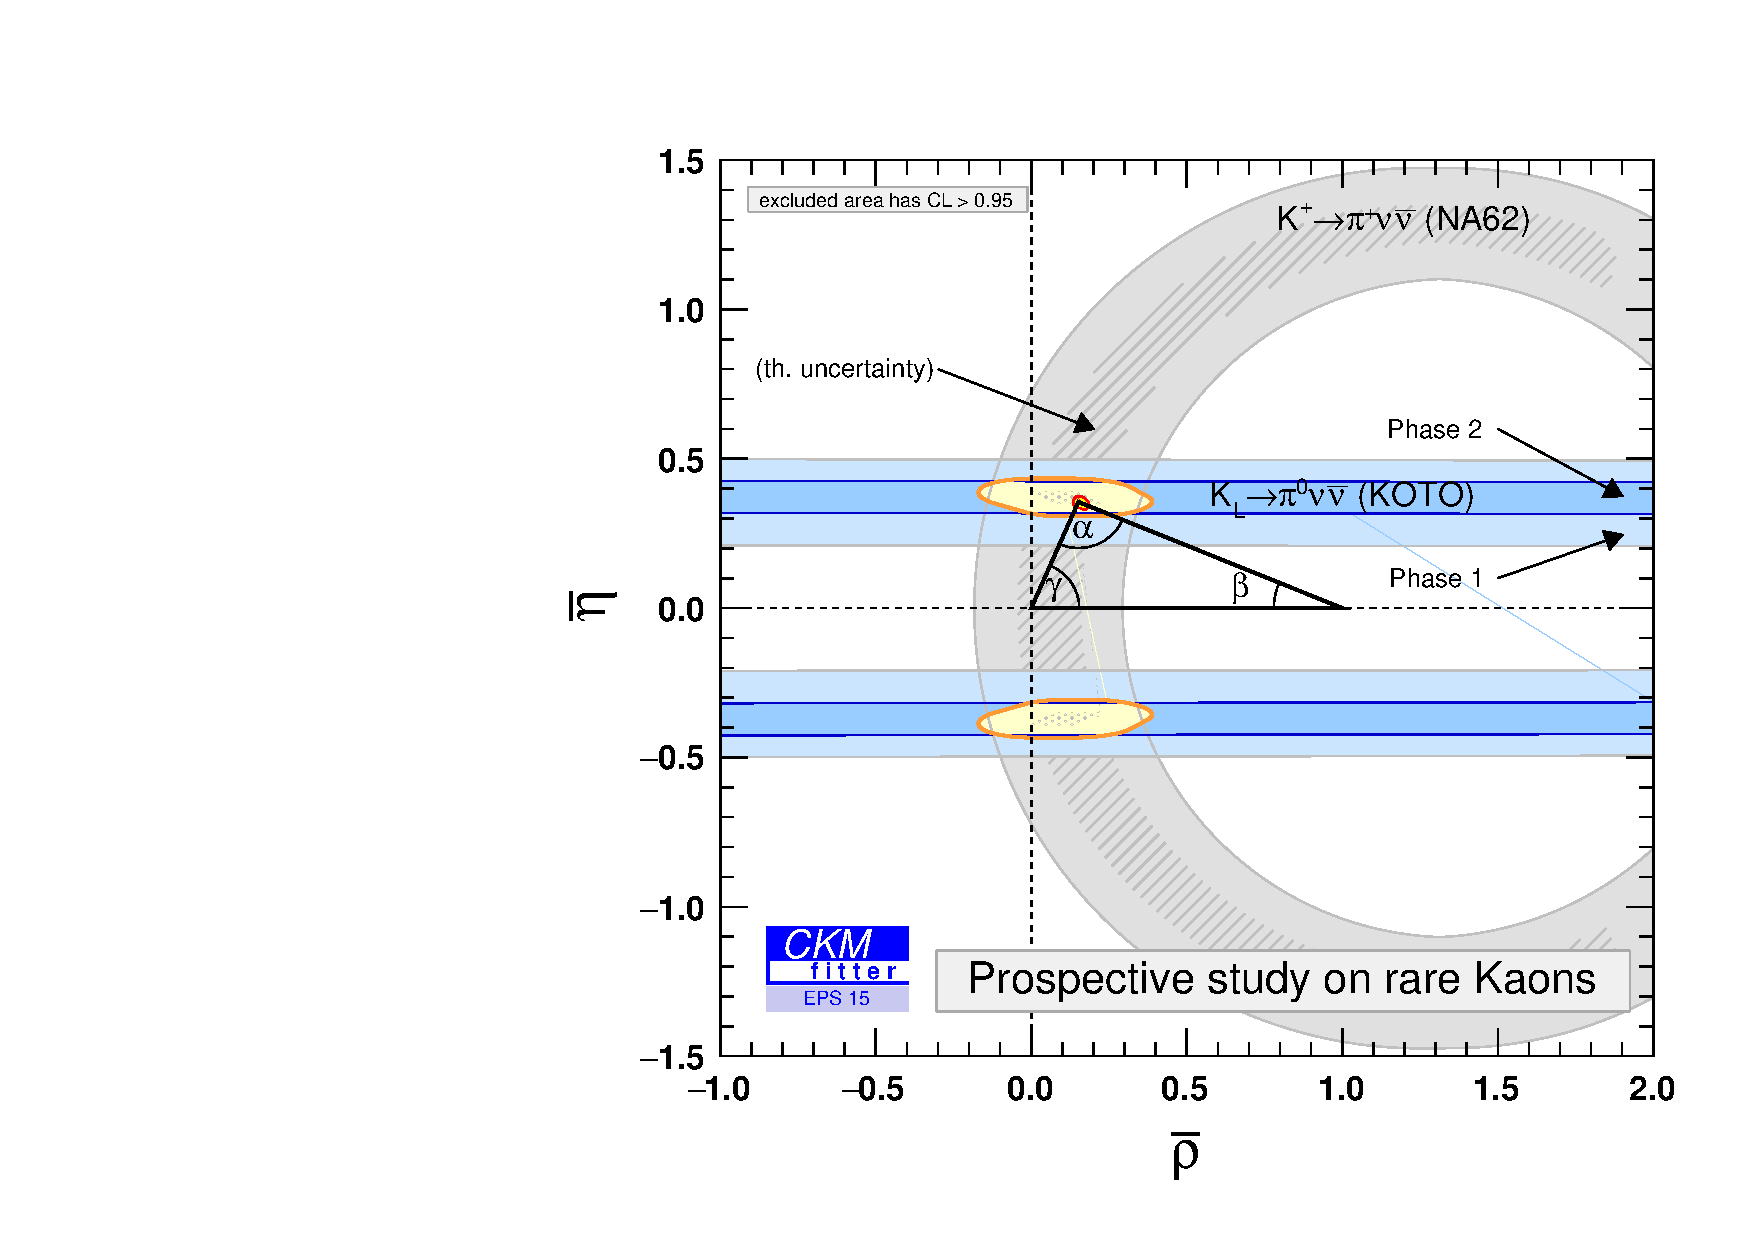
\includegraphics[width=7.5cm]{KbothPibothNuNu_RhoEta.pdf}
\end{center}
\caption{Left plot: summary of the current constraints on direct and indirect $CP$ asymmetry in the charm sector; the overall picture is, with the present uncertainties, consistent with no $CP$ violation observed in the $D$ mesons sector. Right plot: Constraints in the $(\bar{\rho}, \bar{\eta})$ plane, using a prospective scenario for the NA62 and KOTO experiments, from the CKMfitter group . For NA62, a measurement of $\mc B(K^{+}\rightarrow\pi ^{+}\nu\nu)$ with a 10\% accuracy is assumed; for its corresponding constraint (light gray), the theoretical contribution to the uncertainty is indicated by the dashed region. For KOTO, a two-step prospective scenario is assumed: first, a 3$\sigma$ evidence for the $\mc B(K^{+}\rightarrow\pi ^{0}\nu\nu)$ (Phase 1, lighter blue), followed by a later measurement of $\mc B(K^{+}\rightarrow\pi ^{0}\nu\nu)$  with 10\% accuracy (Phase 2, darker blue). For the combined NA62+KOTO constraint, the theoretical contribution to the uncertainty is indicated with the dashed region.}%
\label{fig charm}%
\end{figure}




%\bibliographystyle{JHEP}
%\bibliography{charm_and_K}

%\end{document}
